Describe the RBF-PS method in 2D.

\begin{solution}
    We describe the RBF-PS method in 2D for the Poisson equation on $\Omega = [-1, 1] \times [-1, 1]$ with Dirichlet 
    boundary conditions:

    $$
    \nabla^2 u = f, \quad u(-1, y) = u(1, y) = u(x, -1) = u(x, 1) = 0.
    $$

    To solve this system, we express the discretized 2D Laplacian $L$ as a Kronecker tensor-product so that

    $$
    L = I \otimes A_{\mathcal{L}} + A_{\mathcal{L}} \otimes I
    $$

    where $A_{\mathcal{L}}$ is the previously computed second derivative discretization operator from Problem 3i. We 
    impose boundary conditions explicity by setting the appropriate rows of $L$ to 0 and solving the system

    $$
    L u = f.
    $$

    We implement this strategy in \texttt{problem\_3ii.m} for the forcing function 
    
    $$
    f = \sin{\frac{-5 (x^2 + y^2) \pi^2}{4}}
    $$

    and show the results in Figure \ref{fig:problem_3ii_poisson}.

    \vfill

    \begin{figure}[h]
        \centering
        \begin{subfigure}{0.49\textwidth}
            \centering
            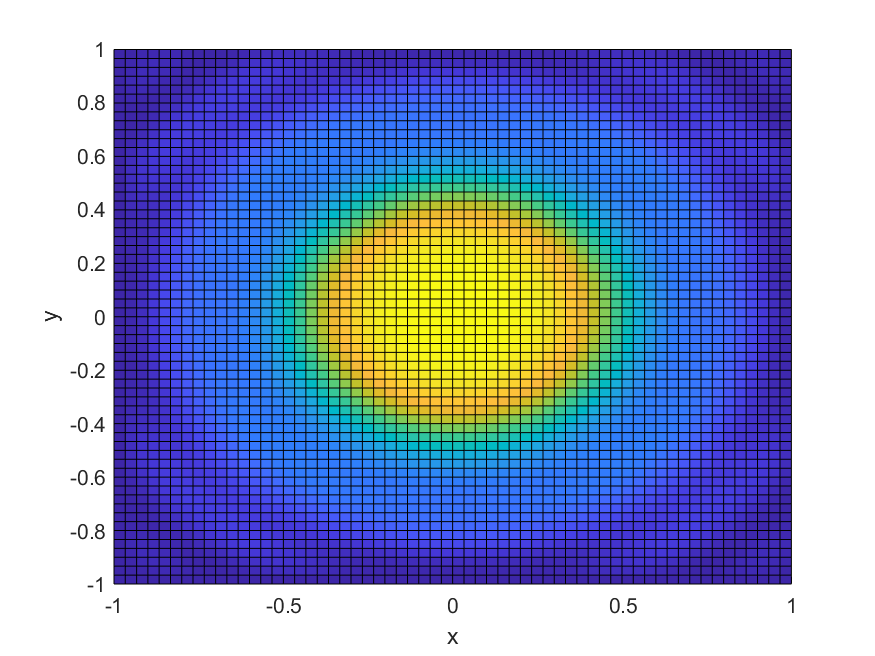
\includegraphics[width=\textwidth]{problem_3ii_poisson_2d.png}
            \caption{2D plot of Poisson equation solution.}
            \label{fig:problem_3i_poisson_2d}
        \end{subfigure}
        \begin{subfigure}{0.49\textwidth}
            \centering
            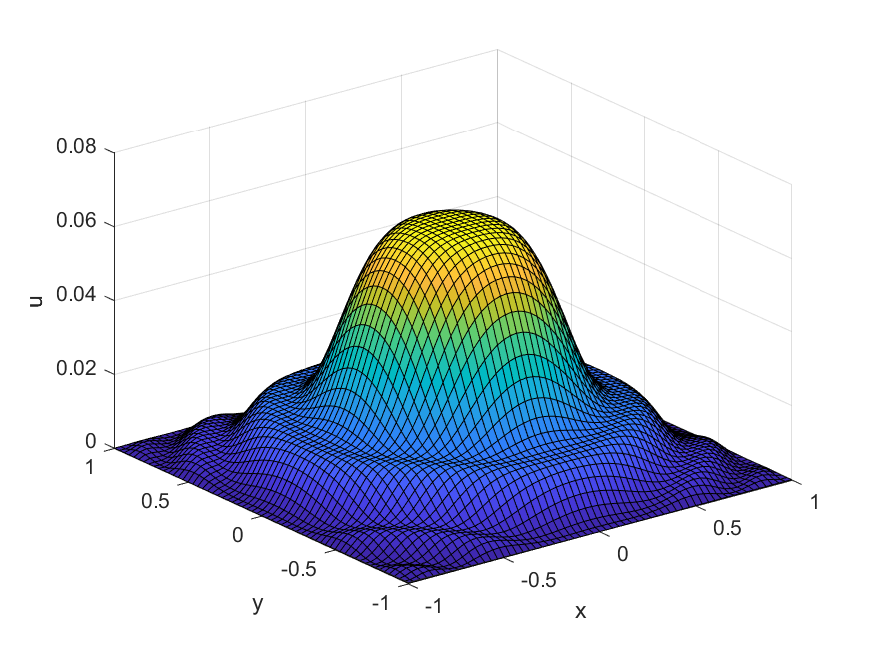
\includegraphics[width=\textwidth]{problem_3ii_poisson_3d.png}
            \caption{3D plot of Poisson equation solution.}
            \label{fig:problem_3i_poisson_3d}
        \end{subfigure}
        \caption{Solution to the 2D Poisson equation using the RBF-PS method.}
        \label{fig:problem_3ii_poisson}
    \end{figure}
\end{solution}